%%%%%%%%%%%%%%%%%%%%%%%%%%%%%%%%%%%%%%%%%
% Focus Beamer Presentation
% LaTeX Template
% Version 1.0 (8/8/18)
%
% This template has been downloaded from:
% http://www.LaTeXTemplates.com
%
% Original author:
% Pasquale Africa (https://github.com/elauksap/focus-beamertheme) with modifications by 
% Vel (vel@LaTeXTemplates.com)
%
% Template license:
% GNU GPL v3.0 License
%
% Important note:
% The bibliography/references need to be compiled with bibtex.
%
%%%%%%%%%%%%%%%%%%%%%%%%%%%%%%%%%%%%%%%%%

%----------------------------------------------------------------------------------------
%	PACKAGES AND OTHER DOCUMENT CONFIGURATIONS
%----------------------------------------------------------------------------------------
\documentclass{beamer}
%\documentclass[handout]{beamer}

\usepackage{mathtools}
\usepackage{comment}

\usetheme{focus} % Use the Focus theme supplied with the template
% Add option [numbering=none] to disable the footer progress bar
% Add option [numbering=fullbar] to show the footer progress bar as always full with a slide count

% Uncomment to enable the ice-blue theme
%\definecolor{main}{RGB}{92, 138, 168}
%\definecolor{background}{RGB}{240, 247, 255}

\definecolor{mygreen}{RGB}{0, 128, 0}
\definecolor{myblue}{RGB}{51, 51, 204}
\definecolor{myviolet}{RGB}{255, 0, 255}

\newcommand{\red}[1]{\textcolor{red}{#1}}
\newcommand{\green}[1]{\textcolor{mygreen}{#1}} 
\newcommand{\blue}[1]{\textcolor{myblue}{#1}}
\newcommand{\violet}[1]{\textcolor{myviolet}{#1}}

\newcommand{\R}{\mathbb{R}}
\newcommand{\Rn}[1][n]{\mathbb{R}^{#1}}
\newcommand{\bx}{\textbf{x}}
\newcommand{\by}{\textbf{y}}
\newcommand{\bz}{\textbf{z}}
\newcommand{\bu}{\textbf{u}}
\newcommand{\bv}{\textbf{v}}
\newcommand{\I}{\mathcal{I}}


%------------------------------------------------

\usepackage{booktabs} % Required for better table rules
\usepackage{slashbox}
\usepackage{ulem,centernot}


%----------------------------------------------------------------------------------------
%	 TITLE SLIDE
%----------------------------------------------------------------------------------------

\title{Cooperative game theory}

\author{Richard Mužík}

%\titlegraphic{\includegraphics[scale=1.25]{Images/focuslogo.pdf}} % Optional title page image, comment this line to remove it

\institute{richard@imuzik.cz}


%------------------------------------------------

\begin{document}

%------------------------------------------------

\begin{frame}
	\maketitle % Automatically created using the information in the commands above
\end{frame}


\begin{comment}
    - Představit kooperativní hru
    - Cíl: Rozdělení zisku v(N)
    - payoff vektor, imputace
    - jádro (důraz na koaliční racionalitu, tj. vysvětlit, proč je jádro stabilní solution concept)
    - Shapleyho hodnota (pomocí formule i axiomů)
    - třídy her (monotonní, superadditivní, konvexní) a jejich vztahy
\end{comment}

%----------------------------------------------------------------------------------------
%	 SECTION 1
%----------------------------------------------------------------------------------------

\section{Introduction} % Section title slide, unnumbered

%------------------------------------------------

\begin{frame}{Cooperative game}
    \begin{block}{Cooperative game}
		\pause
        A \textbf{cooperative game} is an ordered pair $(N,v)$, where $N$ is a set of players and $v\colon 2^N \to \mathbb{R}$ is the characteristic function. Further, $v(\emptyset) = 0$.
    \end{block}
    \begin{itemize}
        \item<5-> $\Gamma^n$ ... set of $n$-person cooperative games
        \item<3-> $S \subseteq N$ ... coalition
        \item<4-> $v(S)$ ... value of coalition
        \item<6-> usually $N = \{1,\dots,n\}$
        \begin{itemize}
            \item<7-> $(S,v_S)$ is \textbf{subgame} $(N,v)$:
            \begin{itemize}
                \item<7-> $v_S \colon 2^S \to \mathbb{R}$
                \item<7-> $v_S(T) \coloneqq v(T)$ pro $T \subseteq S$
            \end{itemize}
        \end{itemize}
    \end{itemize}
	
\end{frame}

%------------------------------------------------

\begin{comment}

%------------------------------------------------

\begin{frame}{Cooperation - examples of models: \textit{Market games}}
	Goal of model? \textit{Understanding of the behaviour of markets}
	\begin{block}{Market}
	   A \textbf{market} $(N,\mathbb{R}^m_+,A,w)$ is given by:
	\begin{itemize}
		\item<2-> $N$ ... set of players
		\item<3-> $\mathbb{R}^m_+$ ... comodity space
		\item<4-> $A \in \mathbb{R}^{m \times n}$ ... matrix of initial allocations
		\begin{itemize}
		    \item<5-> $A = \begin{pmatrix} \mid & \mid & & \mid \\ a^1 & a^2 & \dots & a^n \\ \mid & \mid &  & \mid \\\end{pmatrix}$
			\item<6-> $a^i \in \mathbb{R}^m$ ... commodities owned by player $i$
		\end{itemize}
			\item<7-> $w = w_1 \times w_2 \times \dots w_n$ ... utility function
		\begin{itemize}
			\item<8-> $w_i \colon \mathbb{R}^m_+ \to \mathbb{R}$ ... utility function of player $i$
			\item<9-> $w_i$ is continuous, concave function
		\end{itemize}
	\end{itemize}
	\end{block}
\end{frame}

%------------------------------------------------

%------------------------------------------------

\begin{frame}{Cooperation - examples of models: \textit{Market games}}
	Market games are \textbf{transferable utility} games
	\begin{itemize}
		\item<2-> better understanding after we define cooperative games
		\item<2-> meanwhile: \textit{money} used for evaluation of profit
		\item<3-> formally: $W_i(x,\zeta) = w_i(x) + \zeta$
		\begin{itemize}
			\item<4-> $x \in \mathbb{R}^m$ ... vector of commodities
			\item<4-> $\zeta \in \mathbb{R}$ ... money
			\begin{itemize}
                \item<5-> $\zeta$ may be negative
				\item<5-> amount we paid to buy the commodities
			\end{itemize}
		\end{itemize}
	\end{itemize}
\end{frame}

%------------------------------------------------

%------------------------------------------------

\begin{frame}{Cooperation - examples of models: \textit{Market games}}
	Goal of market games? Determine \textit{trade} on the market
	\begin{block}{Trade of coalition $S$}
		\textbf{Trade} for market $(N,\mathbb{R}^n_+,A,w)$ between players in $\emptyset \neq S \subseteq N$ is a collection $(x^i,\zeta^i)_{i \in S}$ satisfying:
		\begin{enumerate}
                \pause
			\item $\sum_{i \in S}x^i = \sum_{i \in S}a^i$ (preservation of commodities)
                \pause
			\item $\sum_{i \in S}\zeta^i = 0$ (preservation of money).
		\end{enumerate}
	\end{block}
        \pause
	Questions:
        \pause
	\begin{itemize}
            \pause
		\item Which coalitions agree on trading?
		\pause
            \item What trade will occur within a given coalition? 
		\begin{itemize}
			\item \textit{What is the profit of player \textbf{i} for a given market?}
		\end{itemize}
	\end{itemize}
	
\end{frame}

%------------------------------------------------

\end{comment}

%------------------------------------------------

\begin{frame}{Cooperation - examples of models:\\ \textit{Minimal spanning-tree games}}
	Goal: \textit{Find the best connection of players to a source}
	\begin{itemize}
		\item<2-> $N = N' \cup \{0\}$ ... set of players + source
		\item<3-> $c_{ij}$ ... cost of connecting $i,j$
		\item<4-> solution: a network, where each $i \in N$ is connected to $0$ with minimal sum of costs
	\end{itemize}
	
\end{frame}


%------------------------------------------------

\begin{comment}
    

%------------------------------------------------

\begin{frame}{Cooperation - examples of models: \textit{Market games}}
 	\begin{itemize}
 		\item $(N,\mathbb{R}^m_+,A,w)$ ... market
	\end{itemize}
	\begin{block}{Feasible S-allocation}
		\textbf{Feasible $S$-allocations} is $(a_S^i)_{i \in S}$ satisfying
		\[
		\sum_{i \in S}a^i_S = \sum_{i \in S}a^i.
		\]
		We denote the set of feasible $S$-allocations by $\mathcal{A}_S$.
	\end{block}
\end{frame}

%------------------------------------------------

%------------------------------------------------

\begin{frame}{Cooperation - examples of models: \textit{Market games}}
	\begin{itemize}
		\item $(N,\mathbb{R}^m_+,a,w)$ ... market
	\end{itemize}
	\begin{block}{Feasible S-allocation}
		\textbf{Feasible S-allocation} is $(a_S^i)_{i \in S}$ satisfying $\sum_{i \in S}a^i_S = \sum_{i \in S}a^i$.\\
		We denote the set of feasible $S$-allocations by $\mathcal{A}_S$.
	\end{block}
	\begin{block}{Market game}
		Cooperative game $(N,v)$ is \textbf{market game}, if there is market $(N,\mathbb{R}^m_+,A,w)$ satisfying
		\[
		v(S) = \max\{\sum_{i \in S}w^i(a_S^i)\mid (a_S^i)_{i \in S} \in \mathcal{A}_S\}.
		\]
	\end{block}
\end{frame}

%------------------------------------------------

\end{comment}

%------------------------------------------------

\begin{frame}{Goal of the model of cooperative games}
	\textit{Money first!}
	\vspace{0.3in}
	\begin{itemize}
	    \item<2-> \textbf{Payoff vector} $\bx \in \Rn$
	    \begin{itemize}
	        \item<2-> $x_i$ represents payoff of player $i$
	    \end{itemize}
	    \item<3-> Vector $\bx \in \Rn$ is \textbf{efficient}, if $\sum_{i \in N}x_i = v(N)$
	    \begin{itemize}
	        \item<4-> Usually, we distribute $v(N)$
            \begin{enumerate}
                \item<4-> \textit{value of cooperation} $v(N)$
                \item<4-> \textit{shared costs} $c(N)$
            \end{enumerate}
	    \end{itemize}
	    \item<5-> Vector $\bx \in \Rn$ is \textbf{individually rational}, if $x_i \geq v(i)$
	    \begin{itemize}
	        \item<6-> players prefer $x_i$ over $v(i)$
	    \end{itemize}
	    \end{itemize}
	    \vspace{0.2in}
	    \begin{itemize}
	    \item<7-> $\I^*(v) = \left\{x \in \Rn \mid x(N) = v(N) \right\}$ ... \textbf{preimputation}
	    \begin{itemize}
	        \item<7-> $x(S)\coloneqq \sum_{i \in S} x_i$
	    \end{itemize}
	    \item<8-> $\I(v) = \left\{x \in \I^*(v) \mid \forall i \in N: x_i \geq v(i)\right\}$ ... \textbf{imputation}
	\end{itemize}
\end{frame}

%------------------------------------------------

\section{Solution concepts}

%------------------------------------------------

\begin{frame}{Solution concepts}
	\begin{itemize}
	    \item<2-> Set of payoff vectors satisfying further properties are \textbf{solution concepts}
	    \item<3-> Can reflect payoff distribution, which is
	    \begin{itemize}
	        \item<4-> \textit{...fair...}
	        \item<4-> \textit{...non-discriminatory...}
	        \item<4-> \textit{...stable (players will accept it)...} 
	        \item<4-> \textit{...}
	    \end{itemize}
	\end{itemize}
\end{frame}

%------------------------------------------------

%------------------------------------------------

\begin{frame}{Solution concepts}
    Formally:
	\begin{enumerate}
	    \item<2-> sets of payoff vectors 
	    \begin{itemize}
	        \item<3-> $\Sigma(v) = \left\{x \in \Rn \mid \dots\right\}$
	    \end{itemize}
	    \item<4-> functions on games
	    \begin{itemize}
	        \item<5-> $\Sigma \colon \Gamma^n \to 2^{\Rn}$
	    \end{itemize}
	\end{enumerate}
\end{frame}

%------------------------------------------------

%------------------------------------------------

\begin{frame}{Solution concepts}
    Formally:
	\begin{enumerate}
	    \item sets of payoff vectors
	    \begin{itemize}
	        \item $\Sigma(v) = \left\{x \in \Rn \mid \dots\right\}$
	    \end{itemize}
	    \item functions on games
	    \begin{itemize}
	        \item $\Sigma \colon \Gamma^n \to 2^{\Rn}$
	    \end{itemize}
	\end{enumerate}
	We distringush
	\begin{enumerate}
	    \item<2-> \textbf{single-point} solution concepts
	    \begin{itemize}
	        \item<3-> as a set: $\Sigma(v) = \{x\}$ 
	        \begin{itemize}
	            \item<3-> we prefer: $\Sigma(v) = x$
	        \end{itemize}
	        \item<4-> as a function: $\Sigma \colon \Gamma^n \to \mathbb{R}$
	    \end{itemize}
	    \item<2-> \textbf{multi-point} solution concepts
	\end{enumerate}
\end{frame}

%------------------------------------------------

%------------------------------------------------

\begin{frame}{Multi-point solution concept: The core}
    Idea: \textit{Payoff distribution leads to cooperation...}
	\pause
    \begin{block}{The core}
		\pause
    	For a cooperative game $(N,v)$, the \textbf{core} $\mathcal{C}(v)$ is
    	\[\mathcal{C}(v) = \left\{x \in \I^*(v) \mid x(S) \geq v(S), \forall S \subseteq N \right\}.\]
    \end{block}
    \begin{itemize}
        \item<4-> assumption: \textit{homo economicus} 
        \begin{itemize}
            \item<5-> model of human as a player
            \item<5-> strictly rational and selfish
            \item<5-> follows his subjective goals
        \end{itemize}
        \item<6-> $v(N)$ ... value, which is distributed among players
        \item<7-> $x(S) > v(S) \implies$ coalition $S$ does not leave $N$ 
        \begin{itemize}
            \item<8-> would lead to $(S,v_S)$
            \item<8-> $v(S)$ ... distributed value
        \end{itemize}
    \end{itemize}
\end{frame}

%------------------------------------------------

%------------------------------------------------

\begin{frame}{Multi-point solution concept: The core}
    \begin{block}{The core}
    For a cooperative game $(N,v)$, the \textbf{core} $\mathcal{C}(v)$ is
    \[\mathcal{C}(v) = \left\{x \in \I^*(v) \mid \textcolor{blue}{x(S)} \geq \textcolor{red}{v(S)}, \forall S \subseteq N \right\}.\]
    \end{block}
	\pause
    Reminder
    \begin{block}{Nash equilibrium}
		\pause
		Strategy profile $(s_1,\dots,s_n)$ is \textbf{Nash equilibrium}, if it holds for every player $i$,
		\[
			v_i(s_1,\dots,s_{i-1},\textcolor{blue}{s_i},s_{i+1},\dots,s_n) \geq v_i(s_1,\dots,s_{i-1},\textcolor{red}{t_i},s_{i+1},\dots,s_n)
		\]
		for every $\textcolor{red}{t_i} \in S_i$.
	\end{block}
\end{frame}

%------------------------------------------------

%------------------------------------------------

\begin{frame}{Multi-point solution concept: The core}
    \begin{block}{The core}
    For a cooperative game $(N,v)$, the \textbf{core} $\mathcal{C}(v)$ is
    \[\mathcal{C}(v) = \left\{x \in \I^*(v) \mid x(S) \geq v(S), \forall S \subseteq N \right\}.\]
    \end{block}
    \begin{block}{Emptyness of the core}
		\pause
        There are cooperative games $\left(N,v\right)$ with empty core.
    \end{block}
    \begin{itemize}
        \item<3-> Non-esential games
        \begin{itemize}
            \item<4-> $v\left(N\right) < \sum_{i \in N}v\left(i\right)$
        \end{itemize}
        \item<5-> Let $x \in \mathcal{C}\left(v\right)$
        \begin{itemize}
            \item<6-> $x\left(N\right)=v\left(N\right)<\sum_{i\in N}\leq x\left(N\right)$ 
        \end{itemize}
        \item<7-> $x$ does not exist $\implies$ $C\left(v\right)=\emptyset$
    \end{itemize}
\end{frame}

%------------------------------------------------

%------------------------------------------------

\begin{frame}{Multi-point solution concept: The core}
    Question: \textit{When is the core non-empty?} \\ \pause
	We can encode the core as linear program (P) and determine the dual program (D)
    \begin{itemize}
		\item<3-> $\left(P\right)=\begin{cases}
			min_{x \in \R^n} & x \left(N\right) \\
			\text{subject to} &x\left(S\right) \geq v\left(S\right)\text{ for }S \subseteq N
		\end{cases}$
		\item<4-> $\left(D\right)=\begin{cases}
			max_{y \in \R_{+}^{\left(2^n-1\right)}} & \sum_{S \subseteq N y_S v\left(S\right)} \\
			\text{subject to} & \sum_{\emptyset \neq S \subseteq N} y_S \mathcal{X}_S = \mathcal{X}_N
		\end{cases}$
	\end{itemize}
	\vspace{1.4in}
\end{frame}

%------------------------------------------------

%------------------------------------------------

\begin{frame}{Multi-point solution concept: The core}
    Question: \textit{When is the core non-empty?} \\ 
	We can encode the core as linear program (P) and determine the dual program (D)
    \begin{itemize}
		\item $\left(P\right)=\begin{cases}
			min_{x \in \R^n} & x \left(N\right) \\
			\text{subject to} &x\left(S\right) \geq v\left(S\right)\text{ for }S \subseteq N
		\end{cases}$
		\item $\left(D\right)=\begin{cases}
			max_{y \in \R_{+}^{\left(2^n-1\right)}} & \sum_{S \subseteq N y_S v\left(S\right)} \\
			\text{subject to} & \sum_{\emptyset \neq S \subseteq N} y_S \mathcal{X}_S = \mathcal{X}_N
		\end{cases}$
	\end{itemize}
	We derive the weak Bondereva-Shapley theorem
	\begin{block}{Weak Bondareva-Shapley theorem}
		Cooperative game $\left(N,v\right)$ has non-empty core if and only if 
		\[
			v\left(N\right) \geq \sum_{S \subseteq N} y_S v\left(S\right)\text{ for all feasible }y \in \R^{\left(2^n-1\right)}
		\]
	\end{block}
\end{frame}

%------------------------------------------------

%------------------------------------------------

\begin{frame}{Single-point solution concept: The Shapley value}
    Idea: \textit{Divide the profit in a fair way...}
	\pause
    \begin{block}{The Shapley value}
		\pause
        For a cooperative game $(N,v)$, the \textbf{Shapley value} $\phi(v)$ of player $i$ is
        \[
        \phi_i(v) = \sum_{S \subseteq N \setminus i}\frac{s!(n-s-1)!}{n!}\left(v(S \cup i) - v(S)\right)
        \]
    \end{block}
    \begin{itemize}
        \item<4-> $v(S\cup i)-v(S)$
        \begin{itemize}
            \item<5-> \textit{marginal contribution} (of player $i$ in $S \cup i$)
        \end{itemize}
        \item<6-> $\frac{s!(n-s-1)!}{n!}$ 
        \begin{itemize}
            \item<7-> weights reflecting different sizes of coalitions
        \end{itemize}
        \item<8-> $\sum_{S \subseteq N \setminus i}$
        \begin{itemize}
            \item<9-> sum of all marginal contributions of $i$
        \end{itemize}
    \end{itemize}
\end{frame}

%------------------------------------------------

%------------------------------------------------

\begin{frame}{Single-point solution concept: The Shapley value}
    Idea: \textit{Divide the profit in a fair way...}
    \begin{block}{The Shapley value}
        For a cooperative game $(N,v)$, the \textbf{Shapley value} $\phi(v)$ of player $i$ is
        \[
        \phi_i(v) = \sum_{S \subseteq N \setminus i}\frac{s!(n-s-1)!}{n!}\left(v(S \cup i) - v(S)\right)
        \]
    \end{block}
    \begin{itemize}
        \item<2-> The players agree om the following procedure:
        \begin{enumerate}
			\item<3-> Form the grandcoalition N.
			\item<4-> Enter the the coalition individually and randomly.
			\item<5-> When player $i$ enters coalition $S$, he receives $v\left(S \cup i\right)-v\left(S\right)$.
		\end{enumerate}
		\item<6-> $s!\left(n-s-1\right)!$ ... number of situations, in which $i$ enters $S$
		\item<7-> $n!$ ... number of all possible ways to construct $N$
		\item<8-> $\phi_i(v)$ ... the average value of player $i$'s payment
    \end{itemize}
\end{frame}

%------------------------------------------------

%------------------------------------------------

\begin{frame}{Shapley value}
    \textit{It is possible to define it using its properties...}
	\pause
    \begin{block}{The Shapley value}
       The \textbf{Shapley value} $\phi(v)$ is the only function $f \colon \Gamma^n \to \mathbb{R}$ satisfying for all games $(N,v),(N,w)$:
        \begin{enumerate}
            \item<3-> (AXIOM OF EFFICIENCE)
            \begin{itemize}
                \item<4-> $\sum_{i \in N}f_i(v) = v(N)$
            \end{itemize}
            \item<3-> (AXIOM OF SYMMETRY)
            \begin{itemize}
                \item<5-> $\forall i,j \in N$ $(\forall S \subseteq N \setminus \{i,j\}: v(S \cup i) = v(S \cup j)) \implies f_i(v) = f_j(v)$
            \end{itemize}
            \item<3-> (AXIOM OF NULL PLAYER)
            \begin{itemize}
                \item<6-> $\forall i \in N$ $(\forall S \subseteq N: v(S) = v(S \cup i)) \implies f_i(v)=0$
            \end{itemize}
            \item<3-> (AXIOM OF ADDITIVITY)
            \begin{itemize}
                \item<7-> $v,w \in \Gamma^n: f(v+w)=f(v)+f(w)$
            \end{itemize}
        \end{enumerate}
        
    \end{block}
\end{frame}

%------------------------------------------------

%------------------------------------------------

\begin{frame}{Weber set}
    \begin{enumerate}
		\item<2-> We fix one construction of $N$
		\begin{itemize}
			\item<3-> $\sigma \in \Sigma_n$ ... represent it by permutation
			\item<3-> $\sigma(i)$ ... the order, in which player i enters the coalition
		\end{itemize}
		\item<4-> We compute player's payments
		\begin{itemize}
			\item<5-> $m^\sigma_v$ ... \textbf{marginal vector}
			\item<5-> $\left(m^\sigma_v\right)_i=v\left(S_{\sigma(i)}\cup i\right)-v\left(S_{\sigma(i)}\right)$
			\begin{itemize}
				\item<5-> $S_{\sigma(i)}= \left\{j \in N \mid \sigma(j) < \sigma(i)\right\}$ ... predecessors of $i$ under $\sigma$
			\end{itemize}
		\end{itemize}
		\item<6-> We consider all combinations
		\begin{itemize}
			\item<7-> $\mathcal{W}(v)=conv\left\{m^{\sigma}_{v}\mid \sigma \in \Sigma_n\right\}$ ... \textbf{Webber set}
		\end{itemize}
	\end{enumerate}
	\begin{itemize}
		\item<8-> It holds: $\phi(v)=\sum_{\sigma \in \Sigma_n} \frac{m^\sigma_v}{n!}$
	\end{itemize}
	\begin{block}{Relation between the Shapley value and the Webber set}<9->
		For a cooperative game $(N,v)$ it holds:
		\[\phi(v) \in \mathcal{W}(v)\]
		Moreover, $\phi(v)$ is the center of gravity of $\mathcal{W}(v)$.
	\end{block}
\end{frame}

%------------------------------------------------

%------------------------------------------------

\begin{frame}{Weber set}
    \textbf{Provable by induction}:
	\begin{block}{The Weber set contains the core}
		For every cooperative game $(N,v)$, it holds $\mathcal{C}(v) \subseteq \mathcal{W}(v)$
	\end{block}
\end{frame}

%------------------------------------------------


\section{Classes of games}

%------------------------------------------------

\begin{frame}{Classes of games}
    \begin{itemize}
		\item<2-> \textbf{monotonic game} \[\left(S \subseteq T \subseteq N\right)\left(v(S) \leq v(T)\right)\]
		\item<3-> \textbf{superadditive game} \[\left(S,T \subseteq N, S \cap T = \emptyset\right)\left(v(S)+v(T) \leq v\left(S \cup T\right)\right)\]
		\item<4-> \textbf{convex game} \[\left(S,T \subseteq N\right)\left(v(S)+v(T) \leq v\left(S \cap T\right)+v\left(S \cup T\right)\right)\]
		\item<5-> \textbf{essential game} \[v(N) \geq \sum_{i \in N} v(i)\]
		\item<6-> \textbf{balanced game} \[\mathcal{C}(v) \neq \emptyset\]
	\end{itemize}
\end{frame}

%------------------------------------------------

%------------------------------------------------

\begin{frame}{Classes of games}
    Question: \textit{What are the relations between them?}
	\pause
	\begin{block}{Balanced and essential}
		Balanced cooperative games are essential.
	\end{block}
	\begin{itemize}
		\item<3-> $(N,v)$ is essential
		\begin{itemize}
			\item<4-> $\mathcal{I}(v)=\left\{x \in \R^n \mid x(N)=v(N)\land \forall i \in N: x_i \geq v(i)\right\} \neq \emptyset$
		\end{itemize}
		\item<5-> $(N,v)$ is balanced
		\begin{itemize}
			\item<6-> $\emptyset \neq \mathcal{C}(v) \subseteq \mathcal{I}(v)$
		\end{itemize}
	\end{itemize}
\end{frame}

%------------------------------------------------

%------------------------------------------------

\begin{frame}{Classes of games}
    Question: \textit{What are the relations between them}
	\begin{block}{Convex and superadditive}
		Convex cooperative games are superadditive.
	\end{block}
	\begin{itemize}
		\item<2-> $(N,v)$ is convex
		\begin{itemize}
			\item<2-> $\left(S,T \subseteq N\right)\left(v(S)+v(T) \leq v\left(S \cap T\right)+v\left(S \cup T\right)\right)$
		\end{itemize}
		\item<3-> $(N,v)$ is superadditive
		\begin{itemize}
			\item<3-> $\left(S,T \subseteq N, S \cap T = \emptyset\right)\left(v(S)+v(T) \leq v\left(S \cup T\right)\right)$
		\end{itemize}
		\item<4-> $S \cap T = \emptyset$
		\begin{itemize}
			\item<4-> $\left(S \cap T\right) = 0$
			\item<4-> $v(S)+v(T) \leq v\left(S \cup T\right)$
		\end{itemize}
	\end{itemize}
\end{frame}

%------------------------------------------------

%------------------------------------------------

\begin{frame}{Classes of games}
	\begin{figure}
		\centering
		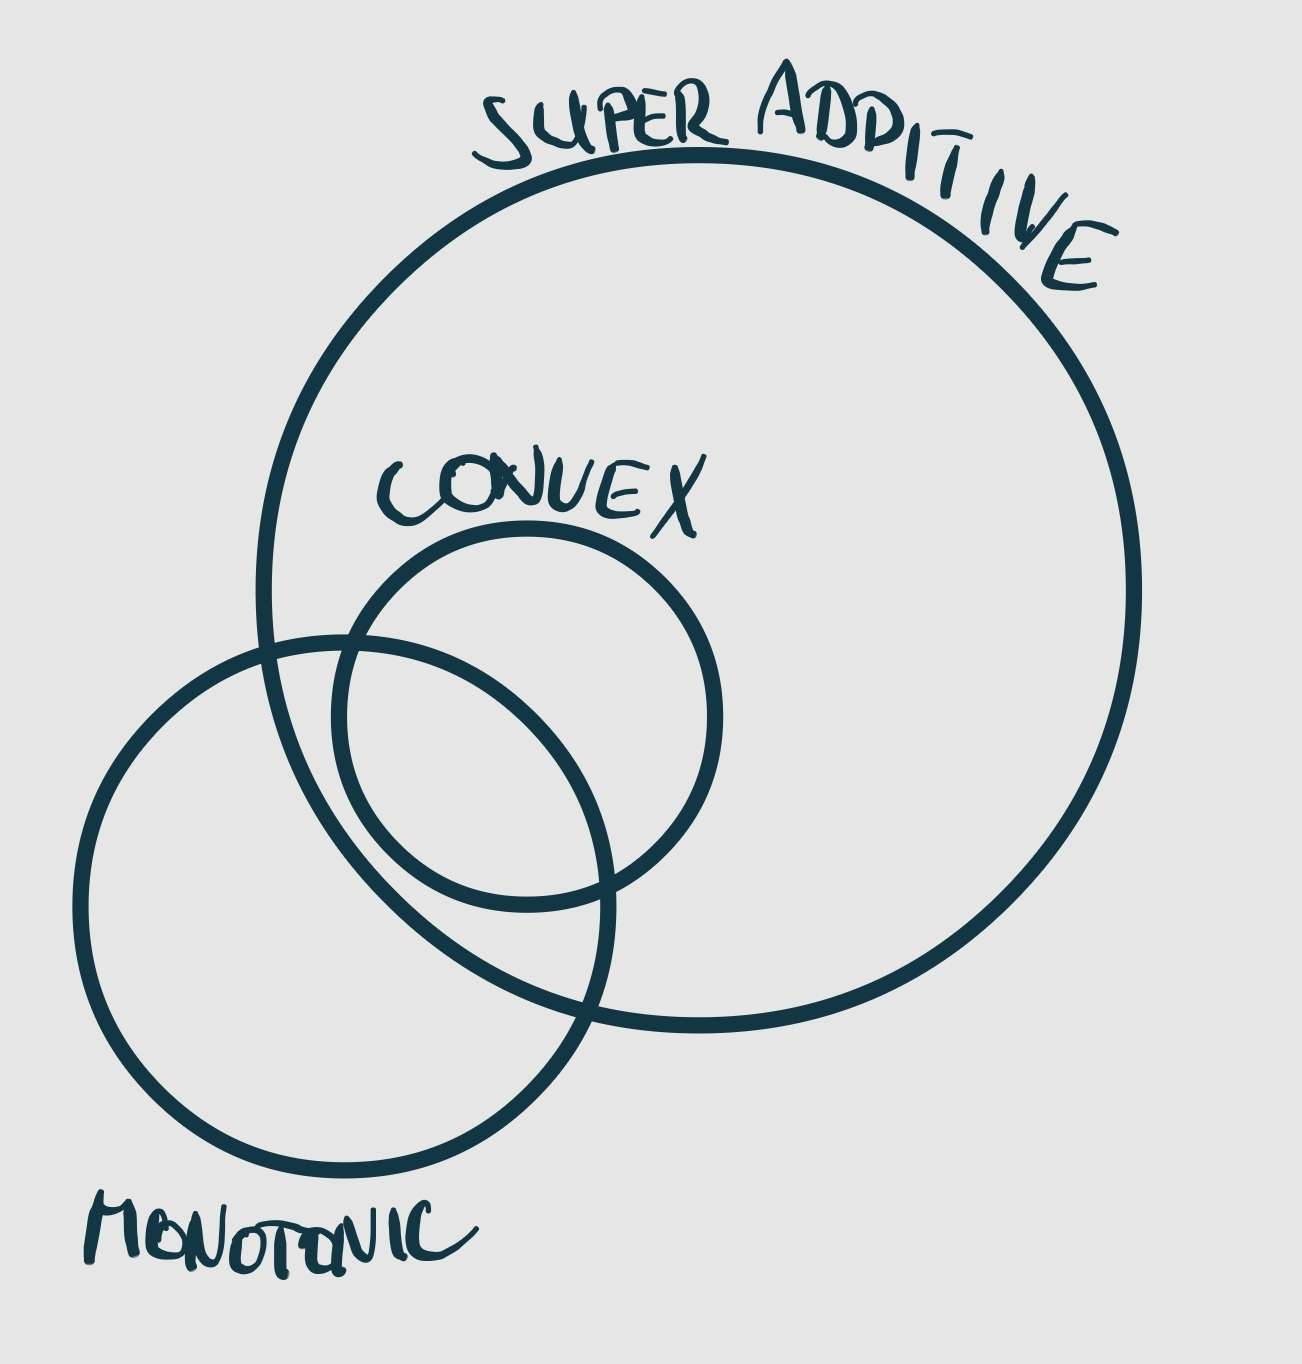
\includegraphics[width=7cm]{Images/classes_of_games.jpg}
	\end{figure}
\end{frame}

%------------------------------------------------

%------------------------------------------------

\begin{frame}{Classes of games}
    \begin{block}{Convex games}
		$\left(S,T \subseteq N\right)\left(v(S)+v(T) \leq v\left(S \cap T\right)+v\left(S \cup T\right)\right)$
	\end{block}
	\pause
	\begin{block}{Core of convex games}
		\pause
		For a convex cooperative game $(N,v)$, it holds $\mathcal{C}(v)=\mathcal{W}(v)$
	\end{block}
	\pause
	Proof: We show only $m^{id}_v \in \mathcal{C}(v)$
	\begin{enumerate}
		\item<5-> $m^{id}_v(N)=\sum_{i \in N} v \left(\left\{1,\dots,i\right\}\right)-v \left(\left\{1,\dots,i-1\right\}\right)=V(N)$
		\item<6-> $m^{id}_v(S) \geq v(S)$
		\begin{itemize}
			\item<7-> $S=\left\{s_1,s_2,\dots,s_k\right\}$
			\begin{itemize}
				\item<7-> $s_1<s_2<\dots<s_k$
			\end{itemize}
			\item<8-> $\textcolor{green}{v (\left\{1,...,s_i\right\})}-\textcolor{blue}{v (\left\{1,...,s_{i-1}\right\})} \geq \textcolor{red}{v (\left\{s_1,...,s_i\right\})}-\textcolor{orange}{v (\left\{s_1,...,s_{i-1}\right\})}$
			\begin{itemize}
				\item<8-> $\left\{s_1,s_2,\dots,s_l\right\} \subseteq \left\{1,\dots,s_l\right\}$ for $l \leq k$
			\end{itemize}
			\item<9-> $m^{id}_v(S)=\sum_{s_i \in S} \textcolor{green}{v \left(\left\{1,\dots,s_i\right\}\right)} - \textcolor{blue}{v \left(\left\{1,\dots,s_{i-1}\right\}\right)}$
			\item<10-> $m^{id}_v \geq \sum_{s_i \in S} \textcolor{red}{v \left(\left\{s_1,\dots,s_i\right\}\right)}-\textcolor{orange}{v \left(\left\{s_1,\dots,s_{i-1}\right\}\right)}=v(S)$
		\end{itemize}
	\end{enumerate}
\end{frame}

%------------------------------------------------

%------------------------------------------------

\begin{frame}{Classes of games}
    \begin{block}{Convex games}
		$\left(S,T \subseteq N\right)\left(v(S)+v(T) \leq v\left(S \cap T\right)+v\left(S \cup T\right)\right)$
	\end{block}
	Consequence:
	\begin{block}{The Shapley value and  convex games}
		\pause
		For a convex cooperative game $(N,v)$, it holds:
		\begin{enumerate}
			\item $\phi(v) \in \mathcal{C}(v)$
			\item $\phi(v)$ is the centre of gravity of $\mathcal{C}(v)$
		\end{enumerate}
	\end{block}
\end{frame}

%------------------------------------------------

\section{Disadvantages of the model and motivation for next lectures}

%------------------------------------------------

\begin{frame}{Disadvantages}
    \begin{block}{Cooperative game}
        A \textbf{cooperative game} is an ordered pair $(N,v)$, where $N$ is a set of players and $v\colon 2^N \to \mathbb{R}$ is the characteristic function. Further, $v(\emptyset) = 0$.
    \end{block}
	\begin{enumerate}
		\item<2-> \textbf{we might not be interested in forming} $N$
		\begin{itemize}
			\item<3-> we want to analyze coalition formation
		\end{itemize}
		\item<4-> \textbf{not every coalition makes sense}
		\begin{itemize}
			\item<5-> two players from completely different fields (why would they want to cooperate)
		\end{itemize}
		\item<6-> $2^n$ \textbf{real values representing} $v$
		\begin{itemize}
			\item<7-> expensive to get all information
			\item<7-> expensive to store all information
		\end{itemize}
	\end{enumerate}
\end{frame}

%------------------------------------------------

%------------------------------------------------

\begin{frame}{Motivation}
    \begin{block}{Cooperative game}
        A \textbf{cooperative game} is an ordered pair $(N,v)$, where $N$ is a set of players and $v\colon 2^N \to \mathbb{R}$ is the characteristic function. Further, $v(\emptyset) = 0$.
    \end{block}
	\begin{enumerate}
		\item \textbf{we might not be interested in forming} $N$
		\begin{itemize}
			\item<2-> games with coalition structure
		\end{itemize}
		\item \textbf{not every coalition makes sense}
		\begin{itemize}
			\item<3-> games on graphs (Martin Černý)
		\end{itemize}
		\item $2^n$ \textbf{real values representing} $v$
		\begin{itemize}
			\item<4-> incomplete games (David Sychrovský + Filip Úradník)
			\item<4-> interval games (Martin Kunst)
			\item<4-> stochastic games (David Ryzák)
			\item<4-> models with compact characteristic function (Martin Černý)
		\end{itemize}
	\end{enumerate}
\end{frame}

%------------------------------------------------

\end{document}
